%------------------------------------------------------------------------------
% Template file for the submission of papers to IUCr journals in LaTeX2e
% using the iucr document class
% Copyright 1999-2013 International Union of Crystallography
% Version 1.6 (28 March 2013)
%------------------------------------------------------------------------------

\documentclass[preprint,pdf]{iucr}              % DO NOT DELETE THIS LINE

     %-------------------------------------------------------------------------
     % Information about journal to which submitted
     %-------------------------------------------------------------------------
     \journalcode{J}              % Indicate the journal to which submitted
                                  %   A - Acta Crystallographica Section A
                                  %   B - Acta Crystallographica Section B
                                  %   C - Acta Crystallographica Section C
                                  %   D - Acta Crystallographica Section D
                                  %   E - Acta Crystallographica Section E
                                  %   F - Acta Crystallographica Section F
                                  %   J - Journal of Applied Crystallography
                                  %   M - IUCrJ
                                  %   S - Journal of Synchrotron Radiation
%\usepackage[format=plain,justification=raggedright,singlelinecheck=false,font=small,labelfont=bf,labelsep=space]{caption}
%\usepackage{lineno}
\usepackage[pdftex]{graphicx}
%\usepackage{epstopdf}
\usepackage{float}

\begin{document}                  % DO NOT DELETE THIS LINE

     %-------------------------------------------------------------------------
     % The introductory (header) part of the paper
     %-------------------------------------------------------------------------

     % The title of the paper. Use \shorttitle to indicate an abbreviated title
     % for use in running heads (you will need to uncomment it).

\title{Online data analysis at ESRF bioSaxs beamline, BM29}
%\shorttitle{Short Title}

     % Authors' names and addresses. Use \cauthor for the main (contact) author.
     % Use \author for all other authors. Use \aff for authors' affiliations.
     % Use lower-case letters in square brackets to link authors to their
     % affiliations; if there is only one affiliation address, remove the [a].

\author[a]{Martha Elisabeth}{Brennich}
\cauthor[a]{J\'er\^ome}{Kieffer}{jerome.kieffer@esrf.fr}{}
\author[a]{Guillaume}{Bonamis}
\author[a,b]{Alejandro}{De Maria Antolinos}
\author[c]{Stephanie}{Hutin}
\author[a]{Petra}{Pernot}
\author[b,c]{Adam}{Round}
\aff[a]{European Synchrotron Radiation Facility, 71 avenue des Martyrs, CS 40220, 38043 Grenoble \country{France}}
\aff[b]{European Molecular Biology Laboratory, Grenoble Outstation, 71 avenue des Martyrs, CS 90181, 38042 Grenoble \country{France}}
\aff[c]{Unit for Virus Host Cell Interactions, Universit\'e Grenoble
Alpes-EMBL-CNRS, 71 avenue des Martyrs, CS 90181, 38042 Grenoble, \country{France}}

     % Use \shortauthor to indicate an abbreviated author list for use in
     % running heads (you will need to uncomment it).

\shortauthor{Brennich, Kieffer et al.}

     % Use \vita if required to give biographical details (for authors of
     % invited review papers only). Uncomment it.

%\vita{Author's biography}

     % Keywords (required for Journal of Synchrotron Radiation only)
     % Use the \keyword macro for each word or phrase, e.g.
     % \keyword{X-ray diffraction}\keyword{muscle}

\keyword{Online data-analysis, solution scattering, protein}

     % PDB and NDB reference codes for structures referenced in the article and
     % deposited with the Protein Data Bank and Nucleic Acids Database (Acta
     % Crystallographica Section D). Repeat for each separate structure e.g
     % \PDBref[dethiobiotin synthetase]{1byi} \NDBref[d(G$_4$CGC$_4$)]{ad0002}

%\PDBref[optional name]{refcode}
%\NDBref[optional name]{refcode}

\maketitle                        % DO NOT DELETE THIS LINE

\begin{synopsis}
Low latency SAXS data reduction for bioSAXS and real time feedback to the users
\end{synopsis}

\begin{abstract}
High throughput small-angle X-ray scattering on proteins in solution at
synchrotron sources is a commonly used technique in structural biology which
relies on highly automated data acquisition.
Data reduction and primary analysis for bioSAXS experiments consists of a
well-defined series of individual tasks the automation of which allows a first
easy assessment of the quality of collected data and the adjustment of
collection strategies if necessary. 
This article describes both the logic and the technical implementation of the
automated processing pipeline for bioSAXS data at the ESRF BM29 beamline using
the EDNA framework.
\end{abstract}


\section{Introduction}
The popularity of small-angle X-ray scattering on proteins and nucleic acids in
solution (bioSAXS) to resolve their three-dimensional shape is continuously
growing \cite{Graewert2013,Hura2009,Reyes2014}.
This has not only resulted in the construction of new dedicated
synchrotron beamlines, such as BM29 at the ESRF, P12 at the EMBL Hamburg or B21
at the Diamond Light Source \cite{BM29paper,P12,B21}, but also pushed forward
new developments in both beamline instrumentation and sample handling.
Examples for this trend are the development of dedicated sample changers
\cite{SCpaper} or the integration of size exclusion chromatography (SEC) systems
into existing beamlines to ensure the mono-dispersity of the sample at a given
time \cite{SECPaper2012,SECP12,SECSWING}.
The \textit{BioSAXS} beamline, BM29, is a small-angle
X-ray scattering beamline dedicated to structural biology \cite{BM29paper}.
Currently, BM29 provides two main experimental modes: 
the use of the
bioSAXS sample changer to collect data on alternating buffer-sample-buffer
sequences (SC mode) and an online HPLC system \cite{SECPaper2012} for
SEC-SAXS experiments (HPLC mode).
In both SC and HPLC mode, data are typically collected at a rate of one frame per second
(1 fps).
In order to estimate the quality of the acquired data, it is
necessary to process them in a quick and robust way, compatible with the
throughput of the beamline.

Available processing tools for SAXS data which support online processing of
large data sets include \textit{DPDAK} \cite{DPDAK}, \textit{bioXTAS raw}
\cite{BioXTASraw}, \textit{SAXSutilities} \cite{SAXSUtilities} and
\textit{SASFLOW} \cite{X33P,P12},  \textit{XRDUA} \cite{xrdua}, \ldots
Most of these either require some advanced input from users or are not open source.
An alternative to these dedicated SAXS tools are more general open source frameworks such as
\textit{EDNA} which is for example used for macromolecular crystallography at
the ESRF \cite{EDNA}.
Our goal was to develop a robust set of online auto-processing pipelines
for bioSAXS experiments, including data reduction, preliminary analysis and
\textit{ab initio} modelling  within the EDNA framework.
The additional needs for flexibility and minimization of
direct user interaction led us to develop pipelines for both SC and HPLC mode
via EDNA.
These pipelines use pyFAI for azimuthal integration \cite{pyFAI} and tools
from the \textsc{atsas} package \cite{ATSAS1,ATSAS2} for analysis and modelling.
Some parts of the \textsc{atsas} package have been re-implemented as a Python
library (named FreeSAS \cite{freesas}) for a better integration into the
Python-based pipeline.
The whole data analysis is smoothly integrated with the beamline control system
(BsxCuBe) and the ISPyBB \cite{ISPYBB} database.


Online data analysis is a key component of any highly automated beamline
where the acquisition of a sample lasts a few seconds and with no dead time
between samples.
Therefore the processing speed must at least keep up with the data acquisition
rate, i.e 1 fps frame per second and about 3 minutes for a set of background and
sample measurements in SC mode.


\subsection{Experiment control}
Data acquisition at the BM29 beamline is controlled via the BsxCuBe
graphical interface, written in Python/Qt4 \cite{pyqt}.
BsxCuBe is composed of control objects which communicate with other beamline
components (i.e. detector, motors, sample changer, data analysis server\ldots)
via the Tango protocol\cite{tango}.

%\subsection{Data analysis server}

%Data analysis is triggered automatically by BsxCube via a tango call.
%The data analysis server is actually a tango device server written in
%PyTango\cite{pytango} which launches EDNA jobs \cite{edna}.


\subsection{EDNA}
EDNA \cite{EDNA} is a plugin-based framework to build pipelines for data-analysis.
Every EDNA-plugin is either responsible
for the execution of a task, i.e. managing an external process,
(called \textit{execution plugins}) or in charge of launching and managing other plugins, either sequentially or in
parallel (called \textit{control plugins}).
The number of execution plugins running simultaneously is limited by the
processor resources of the computer used (and the Python global interpreter
lock).
Any plugin receives its input arguments and returns its result using
EDNA data structures (actually Python objects) which can be serialised into XML
for saving them on the disk or sending them over the network.

An EDNA job is a top level control plugin which communicates with the outside
world, providing its state or its results even after processing is finished,
while keeping its memory footprint as small as possible.

\subsection{The Tango device server}
For accepting processing jobs from the outside, e.g. from the data
acquisition software (BsxCuBe), EDNA provides a Python based Tango device
server interface \cite{tango,pytango}.
The device server starts EDNA jobs via the \textit{startJob} command.
The parameters of this command are the plugin name and the input data structure
associated with it (serialised) and returns a job identifier to the requester.
The Tango device server is hence completely generic and can be used for any
type of EDNA jobs.

To achieve maximum responsiveness at the Tango level, EDNA jobs are not started as
they arrive but they are just instantiated and queued.
Another thread is responsible for starting them and can start multiple jobs in parallel
(data parallelism).
The number of jobs and the number of actual execution
plugins running simultaneously is controlled independently to make the best use
of the computing resources available.

Once finished, every EDNA job produces  a Tango event announcing that the
results are available and also its status: success or failure.
Other processes, e.g. the data acquisition software, can then retrieve the result
of the processing, e.g. the 1D integrated scattering curve and
display it without reading from the disk.
This architecture allows starting processing for individual images or
displaying curves instantaneously without polling the shared file system.
This improves greatly the responsiveness since synchronisation of shared
file systems across the network often exhibits delays of several
seconds.

\subsection{Hardware, software and versions}
Two computers with GP-GPU computing capabilities (Nvidia Quadro 4000) are
dedicated to online data analysis on BM29. 
They are independent and feature the same software installation.
As the \textit{ab initio} reconstruction pipeline lasts dozens of minutes
(due to the final refinement stage using \textit{dammin}), this runs on the
more powerful computer, whereas the azimuthal integration pipeline, which needs
the lowest latency, runs on the smaller computer.
A third computer with similar computing capabilities is available for
\textit{off-line} reprocessing, development of pipelines and acts as a spare.
All three computers are equipped with the Debian 7 operating system and are
used to run \textsc{atsas} (version 2.6.1).



\section{Data analysis pipeline in sample changer mode}

Using the sample changer ensures a high throughput of different samples (
$\sim 3$~min/sample).
Before and after measuring a sample, a background measurement using its
respective buffer is performed.
If the buffer of a sample is the same as the one of the preceding sample, the
background measurement before the sample is skipped.
Hence, data are produced in sequences of the type \textit{buffer 1, sample 1,
buffer 1, buffer 2, sample 2, buffer 2, \ldots}  or  \textit{buffer 1, sample 1,
buffer 1,  sample 2, buffer 1 \ldots}.
Typically for each buffer or sample, 10 frames of 1~s exposure time each are
acquired.

The following steps for data reduction and analysis are required:
\begin{enumerate}
\item the azimuthal integration of an individual frame,
\item the creation of a background-corrected sample scattering curve,
\item basic analysis of the sample scattering curve (Guinier plots, and other
invariants)
\item \textit{ab initio} modelling based on basic analysis.
\end{enumerate}
In the EDNA bioSAXS application (2) and (3) are combined in one pipeline.

\subsection{Azimuthal integration pipeline}
\label{AI}
The azimuthal integration pipeline is triggered for every acquired single frame,
i.e. every second, and thus needs the lowest latency possible to
display the integrated curve in \textit{real time} via BsxCuBe.
The input data structure for azimuthal integration contains
information about the geometry of the experiment, the sample, its concentration
and the transmitted intensity (I1) as measured on the beam-stop diode for
normalisation, etc.
In order to cope with the requested speed (up to 10 frames per second), this
pipeline has been optimised and simplified to a large extent.
It relies on the FabIO \cite{fabio} package for image reading and pyFAI
\cite{pyFAI} for azimuthal integration.
As the images are acquired with a Pilatus 1M pixel detector (manufactured by
Dectris), the error can be assumed to be Poissonian and is integrated as such.
The azimuthal integration is performed on a dedicated graphics card
(Nvidia Quadro 4000) using OpenCL \cite{pyFAI_gpu}, offloading this processing
from CPU to GPU, hence freeing resources for other pipelines.
The subsequent normalisation is performed directly using NumPy~\cite{numpy}.
The result is saved into a 3-column ASCII file (q, I, $\sigma$) for further
processing by the \textsc{atsas} tools \cite{ATSAS2} and sent back to BsxCuBe
for live display.
In accordance with EMBL and ESRF standards, the scattering vector
$q=4\pi\frac{\sin(\theta)}{\lambda}$ is expressed in inverse nanometers.

\subsection{Curve merging, background correction and basic analysis}
\label{SM}
Data acquisition is usually carried out in sets of sample and buffer
measurements.
Each sample or background measurement consists of a set of frames
(typically 10) in order to be able to detect radiation damage
(avoiding the interpretation of data from damaged samples).
The \textit{SmartMerge} pipeline is triggered at the end of each measurement
and is designed to evaluate similarities among scattering
patterns, using the \textit{datcmp} tool from \textsc{atsas} and merging all
similar frames and propagating the associated metadata and
errors.
A flow diagram is depicted in figure~\ref{fgr:smart}.
All curve comparisons can be performed in parallel on modern multicore
computers thanks to the EDNA multi-threaded environment.
Subsequently, the \textit{SmartMerge} plugin averages the individual frames
of a measurement, monitors the buffer-sample-buffer sequence and
 calls the \textit{autoSub} plugin, which determines the optimal buffer
(see below) and subtracts it from the sample data, yielding the 
\textit{subtracted curve} representing only the scattering from the
macromolecule of interest.
If the buffers measured before and after the sample are considered sufficiently
similar by \textit{datcmp} (used to calculate the p-value $p > 0.01$), the
optimal buffer is their average.
If they differ too much ($p \leq 0.01$), each of them is subtracted individually from the
sample curve and the difference resulting in  the smallest radius of
gyration ($R_{G}$), as determined by the tool \textit{autorg} from \textsc{atsas}, is retained.
If both values of $R_{G}$ are identical, the selection is made using the lowest forward scattering intensity $I_{0}$.
If \textit{autorg} fails for both subtracted curves, the buffer with the lowest
total scattering is chosen.
Figure~\ref{fgr:autosub} provides a flow chart of the plugin.

Finally the \textit{subtracted curve} is analysed using the
\textit{SaxsAnalysis} plugin which subsequently applies tools from the
\textsc{atsas} package: the Guinier region fitting using \textit{autorg}, 
the inverse Fourier transform using \textit{datgnom}, 
$p(r)$ and Porod volume assessment using \textit{datprorod}.
In addition the \textit{SaxsAnalysis} plugin creates \textit{PNG} figures of
the subtracted curve and the fitting curve generated by \textit{datgnom}, the
Guinier fit, the $p(r)$ function and Kratky plots whenever possible (Figure~\ref{plots}).
All this information and figures are then directly returned to BsxCuBe to inform
the user of the success of the measurement and additionally logs into the
ISPyBB database \cite{ISPYBB} where the results can be accessed via a web
interface.
Figure~\ref{fgr:analysis} shows a flowchart of the plugin.

\subsection{Ab initio reconstruction pipeline}
\label{abinitio}
Following the analysis pipeline, a three-dimensional dummy atom model based
on the \textit{subtracted curve} is reconstructed.
This pipeline is inspired from a preliminary work
performed at the Diamond Light Source \cite{DiamondSE}.
It runs multiple instances of \textit{dammif} in parallel (8 or 16 by default)
obtaining multiple models \cite{dammif} and benefitting from 
the multi-threading environment of EDNA.
Multiple models give a visual indication of the variations in
reconstruction results and avoid over-interpretation and biased decisions
based on the models.
After a first round of outlier rejections relying on the goodness of fit
($R_{f}$) and the $\chi^{2}$, where the threshold is the mean value plus two
standard deviations, only $N$ valid models remain.

All $N$ remaining models are superimposed two by two using
our open source implementation of \textit{supcomb}, called
\textit{supycomb} which is available freely (MIT license) as part of the
FreeSAS package \cite{freesas}.
Former versions of the pipeline have been using the original
\textit{supcomb} \cite{supcomb} program from \textsc{atsas} by launching
$N*(N-1)/2$ processes in parallel within the EDNA framework.
This turned out to be more advantageous (in terms of speed) to read all models
from disk only once and perform the whole alignment in the memory.
The distance calculation (actually, the normalised spatial discrepancy, NSD)
has been optimised using a binary extension of Python, written in Cython
\cite{cython} and parallelised with OpenMP.
All other transformations rely on NumPy \cite{numpy} code and the geometric
optimisation is performed using the simplex minimizer provided by SciPy
\cite{scipy}.

A table containing the NSD is then generated
(Figure \ref{fgr:nsd}), explaining which model is the nearest among all
other valid models. 
The selected model is called the reference model and all other valid
models are re-oriented and aligned on the reference one.
All models with an NSD higher than the mean plus one standard deviation are
discarded.

All valid models are merged using \textit{damaver} \cite{damaver},
and \textit{damfilt} to get the average solution. 
The \textit{damaver} model is also filtered using \textit{damstart} to flag
core and shell dummy atoms before performing the refinement of the model using
\textit{dammin} \cite{dammin}.
This last step is pretty slow an lasts usually dozens of minutes. 
If it lasts longer then half an hour, we assume that \textit{dammin} will not finish and 
EDNA aborts the process in order to free resources. 
All results are uploaded into the ISPyBB database, where they can also be
visualised. 
Figure~\ref{fgr:modelling} shows a flowchart of the modeling plugin.


\section{Data analysis pipeline in HPLC mode}
While the sample changer makes a high throughput of samples possible, it
requires homogeneous samples which do not degrade.
Protein samples often are intrinsically heterogeneous.
For example, constituents of a complex present in excess or proteins
might aggregate.
One approach to address this issue is to purify the sample directly online by collecting data
on the eluent from a size-exclusion chromatography column (SEC-SAXS or HPLC
mode) \cite{SECPaper2012,SECP12,SECSWING}.
At the BM29 beamline, one continuously collects 2D-diffraction frames
throughout the SEC purification process at a rate of 0.5 to 5 Hz
(depending on the synchrotron filling mode and the duration of the SEC
purification, 1 Hz being the standard rate), resulting in up to a few thousands
frames.
While the first few frames are acquired on the buffer, the sample composition
for successive frames is not known \textit{a priori}.
The result of a SEC-SAXS experiment can be of very difficult interpretation.
Our automatic analysis delivers reduced data and basic analysis for
every individual frame.
In addition, it uses this information to try to identify regions in the
chromatogram which refer to one species and merges frames from these
regions to improve the signal-to-noise ratio.
The goal of this procedure is not to produce an idealised curve of an individual
species but to give a hint on the overall data quality at an early stage of
the experiment.

\subsection{HPLC single frame pipeline}

The HPLC single frame processing pipeline is activated for every frame in HPLC
mode.
It integrates each frame using the azimuthal integration pipeline (see
\ref{AI}) and compares the result to the first frame using the the
\textit{p-value} calculated by \textit{datcmp} from the \textsc{atsas} package.
The frame is then classified as buffer, sample, or ``in between''
according to the \textit{p-value} ($p>0.1$, $0.01 > p$, $0.01>p>0.1$, 
respectively).
The first time a frame in a HPLC run is not classified as buffer, all previous
frames are averaged to yield an ``average buffer''.
For any frame classified as sample, the ``average buffer'' is subtracted, Guinier
analysis is performed (with \textit{autorg} from the \textsc{atsas} package),
delivering a radius of gyration $R_G$ and the forward scattering intensity
$I_0$. The correlated volume is also calculated in order to estimate the
sample mass \cite{RamboTainerNature2013}.
In addition, the total scattering intensity of any
frame is calculated, regardless of the current classification.
These operation occur at about 2 Hz on the current hardware, but often the
acquisition speed is 1 fps, so that the image can be integrated and displayed
almost in real time.


\subsection{HPLC data processing}
When the HPLC experiment ends (or is aborted) a specific plugin
(\textit{HPLC flush}) is launched to finish the processing of the experiment as
one SEC-SAXS run. 
This plugin uses the results of \textit{autorg} to locate peaks using
continuous wave transformation, as implemented in SciPy, on the forward
scattering \cite{cwt,scipy}, and then merges all individual curves around a local maxima
of the forward scattering with similar radii of gyration ($R_G$).
All processing results from the \textit{HPLC single frame pipeline} and the results of
the peak finding are saved into a single HDF5 file which is uploaded into the
ISPyBB database at the end of the data processing flow.
In addition, the same plugin creates figures (in PNG and in SVG format) of 
total scattering, forward scattering and radius of gyration \textit{vs.} frame
number (or time).
Figure \ref{fgr:SEC} shows the result of a HPLC
experiment where one main peak and a trailing shoulder are identified.
All merged files are further analysed by the \textit{SAXS analysis}
(\ref{SM}) and the \textit{ab initio reconstruction pipeline}
(\ref{abinitio}) plugins described in the sample changer section.

\section{Offline data analysis}
In case offline processing is required, e.g. when one of the parameters for
the azimuthal integration of previously processed data needs to be adjusted,
several Python scripts for starting sub-pipelines are available.
These tools are part of the EDNA installation and just instantiate the needed
plugin and run using the parameter description file which has been modified
accordingly.
For the HPLC mode and the curve merging task, specific tools to reprocess (if
needed) complete datasets are available.

The drawback of this approach is that it relies on the EDNA infrastructure, which is
non trivial to install and even more difficult to customize 
(\textsc{atsas} executable path and related licensing issues, number of cores,
GPU configuration, timeouts for any part of the pipelines, \ldots).
The availability of a spare computer on the beamline dedicated to offline
processing removes this need, hence reprocessing never interferes with ongoing
acquisitions.

\section{Practical example}
To illustrate the functionality of the processing pipeline, data from
a ``deletion construct'' of the protein D5 from  Vaccinia virus (VACV)
were acquired both as a dilution series using the sample changer and
using SEC-SAXS (see figures \ref{fgr:SCcurves}, \ref{fgr:SEC} and
\ref{fgr:curves}, respectively).
The online analysis results of the sample changer data indicate concentration effects
as the $R_G$ decreases versus the  sample concentration (see
table~\ref{tbl:results}).
To eliminate potential undesired oligomers (e.g. aggregates), a SEC-SAXS run
was additionally performed.
The total scattering chromatogram generated nearly instantaneously via
BsxCuBe displayed a strong main peak with extended tails on both sides (see
figure \ref{fgr:SEC}).
After the completion of the run, the complete analysis results could be
examined via ISPyBB.
The forward scattering intensity shows the same peak as the total scattering intensity.
The radius of gyration and the mass estimate get systematically
smaller with higher frame numbers, suggesting a larger size component.
Both stabilize with longer elution time (higher frame numbers) and keep 
constant until the end of the peak.
When merging the data, the auto-processing suggested the region highlighted
blue in figure \ref{fgr:SEC}.
For further manual processing and modelling of the protein, the smaller
hashed region was chosen.
Direct comparison of the two merged curves that differ only at the noise
level (figure \ref{fgr:curves}).
By comparing the radius of gyration from the SEC-SAXS data with the data
acquired using the sample changer, a consistently lower $R_G$ is stated (see
table \ref{tbl:results}), whilst a direct comparison of the curves shows a
slightly higher signal at low angles for sample changer data, indicating
the presence of aggregates.

%In our example, the auto-processing helped us to optimize our experiment on the fly.

\section{Conclusions and Outlook}
As illustrated by the example in the preceding section, auto-processing has
become an invaluable tool for experiments at the \textit{bioSaxs} beamline BM29, 
enabling optimization of the
data acquisition parameters to obtain the best data, avoiding the effects of
radiation damage on the data, measuring additional dilutions where inter-particle 
scattering is observed or switching to online SEC where necessary. 
Additionally, where data quality is good enough the auto-processing feedback
allows efficient use of beamtime avoiding additional unnecessary measurements
and giving users the needed confidence to move over to the next highest priority
samples.
The combination of auto-processing software tools and
the presentation of the results in a user-friendly manner in ISPyBB facilitates
experiments for both experienced and novice users by enabling the former to
spend time preparing more samples and acquiring more useful data (instead of
data processing), and the latter to get an easier access to the relevant
beamline techniques.
Auto-processing provides real time feedback on data quality and on the progress 
of the experiment enabling the users to spend more time on scientific insight
and to plan the best experimental strategy.
Additionally the automation of data processing, going hand in hand with
data acquisition, increases the efficiency of an experiment
which may hence be carried out confidently by just one individual.

To further enhance the experiment capabilities, the delay of the feedback to the
user should be kept minimal, providing systematically consistent results.
As of today, the weakest point of all processing pipelines is the
\textit{ab initio} Monte-Carlo modelling which may have abort the
execution of the \textit{dammin} process (often due to a time-out in
the EDNA plugin).
By re-implementing a parallel computation version of this Monte-Carlo modelling
step in FreeSAS, its direct integration into the
EDNA pipeline would maintain the execution time within a couple of minutes,
thus providing faster feed-back to the user.

%The modularity of the EDNA-plugin based approach facilitates the addition of
%new tools as well as the re-use of existing plugins for other purposes. For
%example, it will be easy to add new tools such as \textsc{shanum}
%\cite{SHANUM}, which estimates the number of meaningful Shannon channels,
%without affecting the integrity of the existing pipline.
%Additionally, the existing EDNA plugins can easily be integrated into more
%complex workflows such as those already available for macromolecular
%crystallography \cite{workflow}.

\appendix
\ack{The authors would like to thank Ricardo Fernandes and Thomas Boeglin for developing
the original offline reprocessing tools, Peter Boesecke for the original azimuthal
integration procedure, Olof Svensson for the development of EDNA, Irakli Sikharulidze for
the original version of the \textit{ab initio} modelling pipeline,
Alexey Kikhney, Daniel Franke and Dmitry Svergun for the \textsc{atsas} package
and their support in its implementation, Staffan Ohlsson and Matias Guijarro for
the integration of the data analysis tools into the data acquisition software,
Wim Burmeister for helpful discussions and support, 
Claudio Ferrero, head of ESRF data analysis unit, for the critical revision of
this manuscript.
Stephanie Hutin was financially supported by an ANR grant (REPLIPOX,
ANR-13-BSV8-0014).}


\bibliographystyle{iucr}
\bibliography{biblio}


\section{Preparation of protein sample and data acquisition}
All examples of data in this manuscript are based on a deletion construct of
the D5 protein from vaccinia virus (VACV).
The sequences of D5R are from the VACV strain Copenhagen (GenBank accession
number M35027.1).
D5 391-785 was cloned into the pProEx Htb plasmid (Invitrogen), fused to an N-terminal
TEV(tobacco etch virus) protease-cleavable hexahistidine tag. The protein was expressed in
BL21* and purified over a HIS-select column (Sigma); lysis buffer: 50 mM Tris
pH 8.5, 150 mM NaCl, 5 mM MgCl$_{2}$; complete protease inhibitor cocktail
(Roche), DNaseA, 10 mM beta-Mercaptoethanol; binding buffer: 50 mM Tris pH 8.5, 150 mM NaCl, 10 mM beta-Mercaptoethanol; 
high salt wash buffer: 50 mM Tris pH 8.5, 1 M NaCl, 10 mM beta-Mercaptoethanol; 
elution buffer: 50 mM Tris pH 8.5, 150 mM NaCl,  200 mM imidazole, 10 mM beta-Mercaptoethanol. 
The buffer of the eluates was exchanged to a binding buffer on a PD10 column and
the protein was TEV-digested over night at RT. 
After a second Ni-column, the sample was injected into a 
Superdex 200 GL 10/300 column (GE Healthcare), equilibrated with gel filtration
buffer (20 mM Tris pH 8.5, 150 mM NaCl, 1 mM dithiothreitol, DTT). 
Eluted peaks were analysed by 
SDS-PAGE, stained with InstantBlue (Expedeon).
In SC mode a dilution series of five different concentrations
was prepared (see table~\ref{tbl:results}). 
For size exclusion, 50~$\mu$l of sample at 20~mg/ml on a Superdex
200 5/150 GL column (GE healthcare) were injected.


\section{Software distribution and licensing}

All pieces of software developed for online data analysis at the bioSAXS
beamline are open source.
Nevertheless they rely on the \textsc{atsas} package which, although free
for academic use, is neither open source, nor redistributable.

EDNA is licensed under LGPL for the kernel part (the pipeline engine) and GPL
for the bioSAXS part. The source code is now hosted on a public
repository at:\\
https://github.com/edna-site.\\
EDNA is a server tool for online data analysis and the developers are aware of
how difficult it may be to install and configure it properly. EDNA controls
\textsc{atsas} modules by executing external programs in pipe mode, avoiding
any licensing issues.

The azimuthal integration is performed via pyFAI \cite{pyFAI}, the Python library
for fast azimuthal integration, which is GPU-accelerated \cite{pyFAI_2015}.
Diffraction images are read by the FabIO library \cite{fabio}.
Both libraries are licensed under GPL and hosted under the following web
pages:\\
http://github.com/pyFAI and https://fable.sf.net\\
Some \textsc{atsas} parts have been re-implemented  directly in EDNA  
to offer a better integration into the processing pipelines (by avoiding the
forking of many sub-processes): \textit{dataver}, \textit{datop}, \ldots 
\textit{Supycomb} is available as part of the \textsc{FreeSAS} package which
re-implements the \textit{supcomb} algorithms, featuring a MIT license scheme. 
FreeSAS can be downloaded from
https://github.com/kif/freesas but waiving any numerical equivalence to the
reference implementation.
Finally the other tools of the Python scientific stack (NumPy, SciPy,
Matplotlib) are subjected to the BSD license conditions.


\begin{figure}
\centering
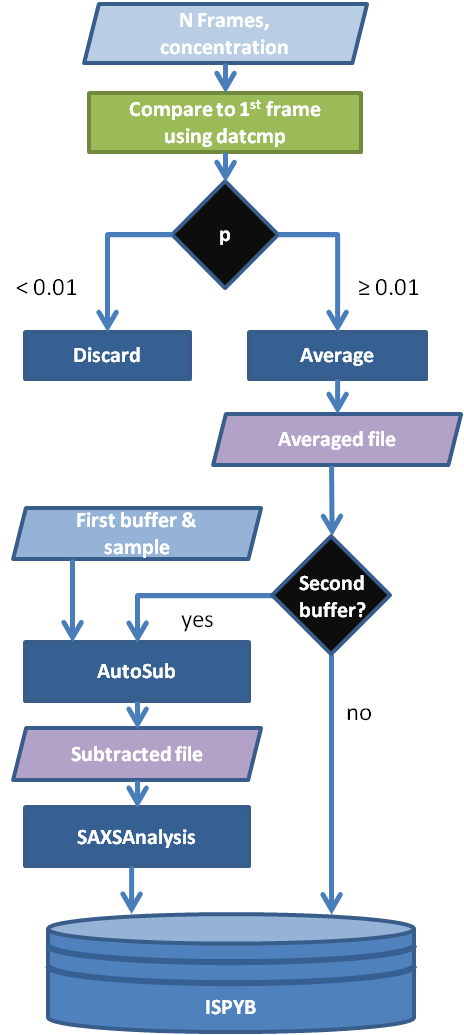
\includegraphics[width=8cm]{smartmerge.png}%
\caption{Flow chart of the \textit{SmartMerge} plugin for data reduction.
This plugin controls the averaging of individual frames and triggers background
subtraction and preliminary analysis if required.
Bright blue parallelograms indicate data input, violet parallelograms data
output, black diamonds decision steps, green rectangles processing using
\textsc{atsas} tools and blue rectangles processing using non-\textsc{atsas} tools. }
\label{fgr:smart}
\end{figure}

\begin{figure}
\centering
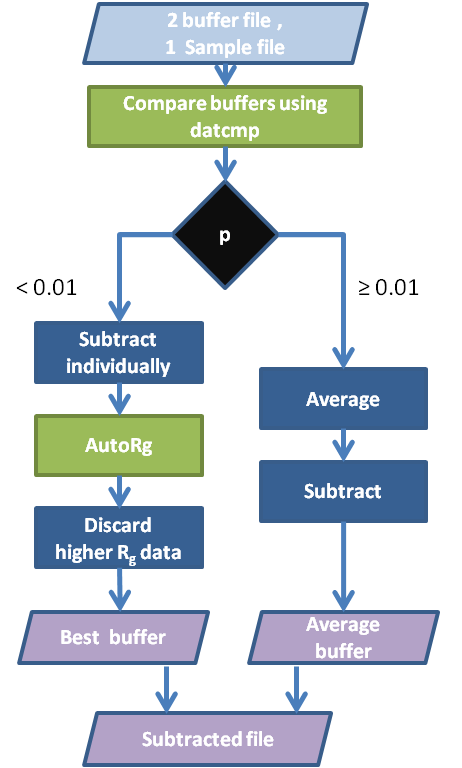
\includegraphics[width=8cm]{autosub.png}%
\caption{Flow chart of the \textit{autoSub} plugin for subtracting the ``best''
buffer.
This plugin subtracts the background from the total scattering signal after
selecting the most suitable buffer.
Symbols are those described in figure \ref{fgr:smart}.}
\label{fgr:autosub}
\end{figure}

\begin{figure}
\centering
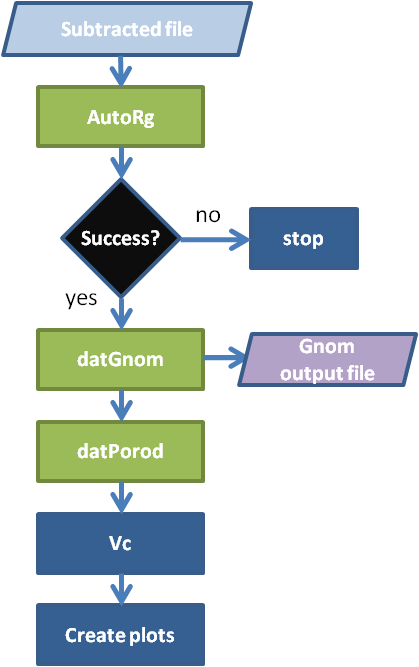
\includegraphics[width=8cm]{analysis.png}%
\caption{Flow chart of the \textit{saxsAnalysis} plugin.
This plugin applies various preliminary analysis methods to background
corrected data.
Symbols are those described in figure \ref{fgr:smart}.}\label{fgr:analysis}
\end{figure}

\begin{figure}
\centering
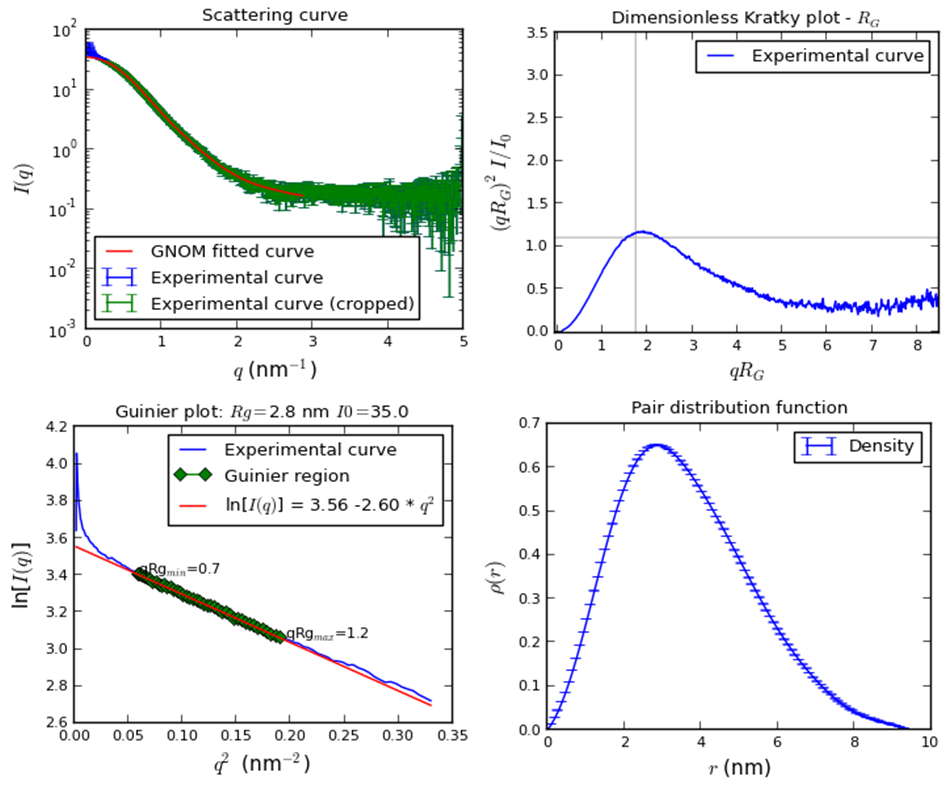
\includegraphics[width=18cm]{autoplot.png}
\caption{Examples of the curves automatically generated by the
\textit{SaxsAnalysis} pipeline: scattering curve (top left), normalized Kratky
plot (top right), Guinier plot (lower left) and pair distribution function
The layout results from an adjustment of the standard version for
improved readability of the printouts.}
\label{plots}
\end{figure}

\begin{figure}
\centering
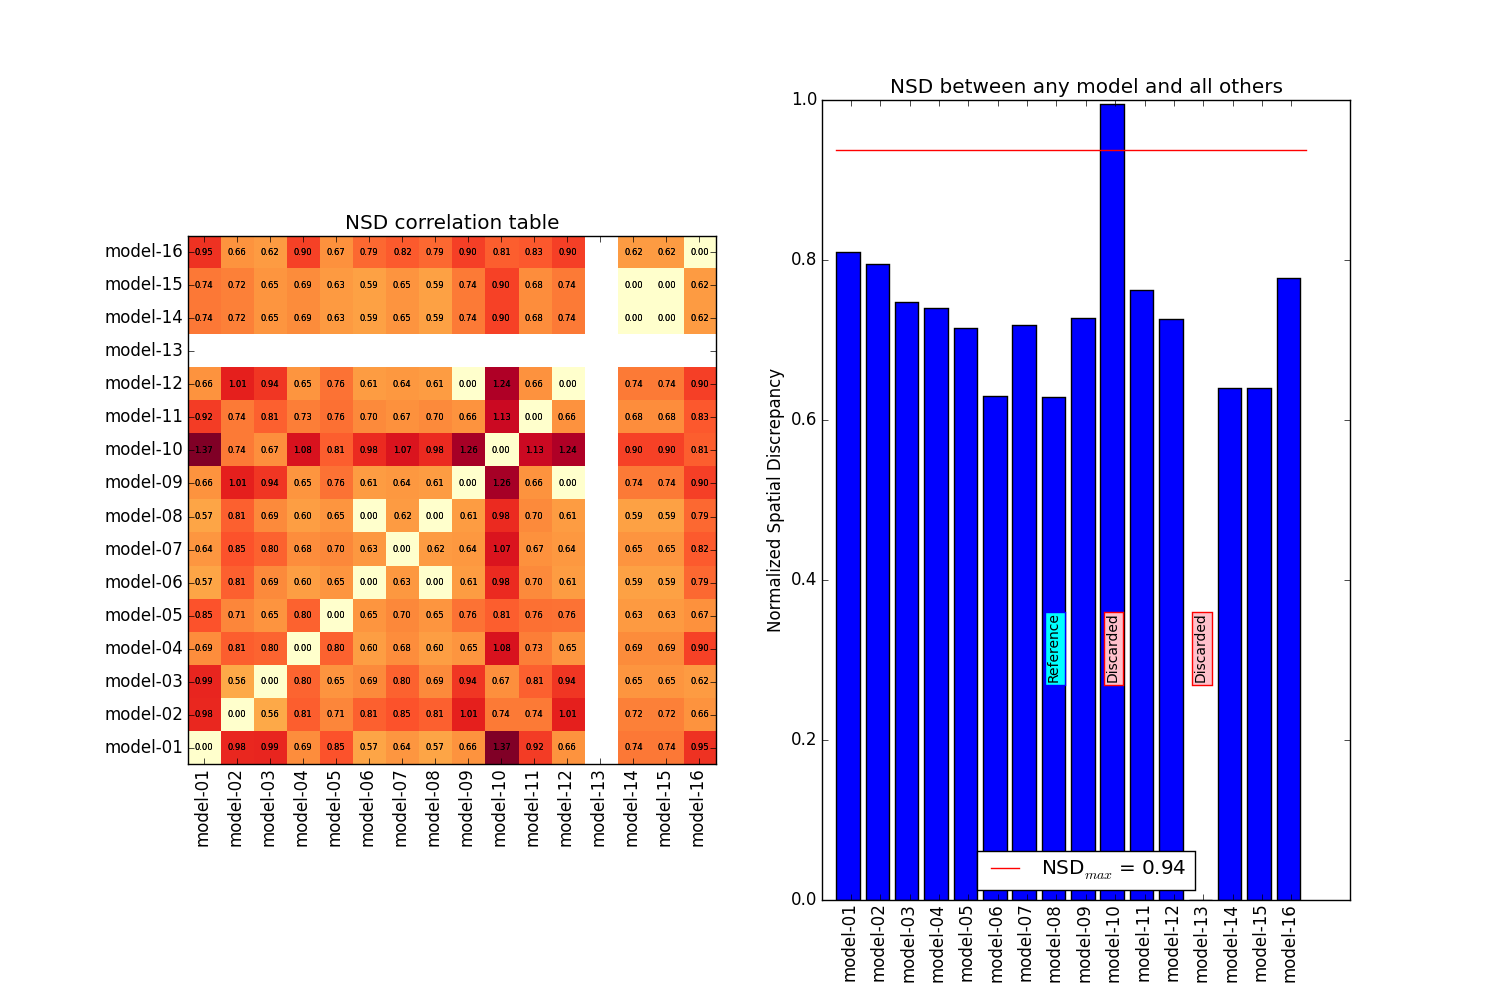
\includegraphics[width=18cm]{nsd.png}
\caption{Plots created by the \textit{supycomb} program for comparing a set
of \textit{ab initio} models.
The matrix on the left hand-site represents the pair-wise normalised spatial
discrepancy (NSD) between two models.
The bar plot on the right hand-site reproduces the mean NSD.}
\label{fgr:nsd}
\end{figure}

\begin{figure}
\centering
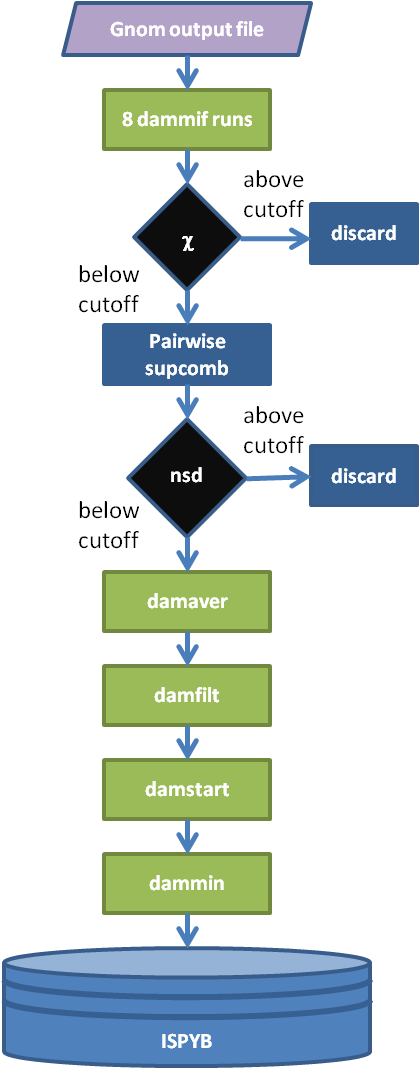
\includegraphics[width=8cm]{model.png}
\caption{Flow chart of the \textit{ab initio} reconstruction plugin from a
\textit{gnom} file (pair distance distribution function).
Symbols are those described in figure \ref{fgr:smart}.}\label{fgr:analysis}
\label{fgr:modelling}
\end{figure}

\begin{figure}
\centering
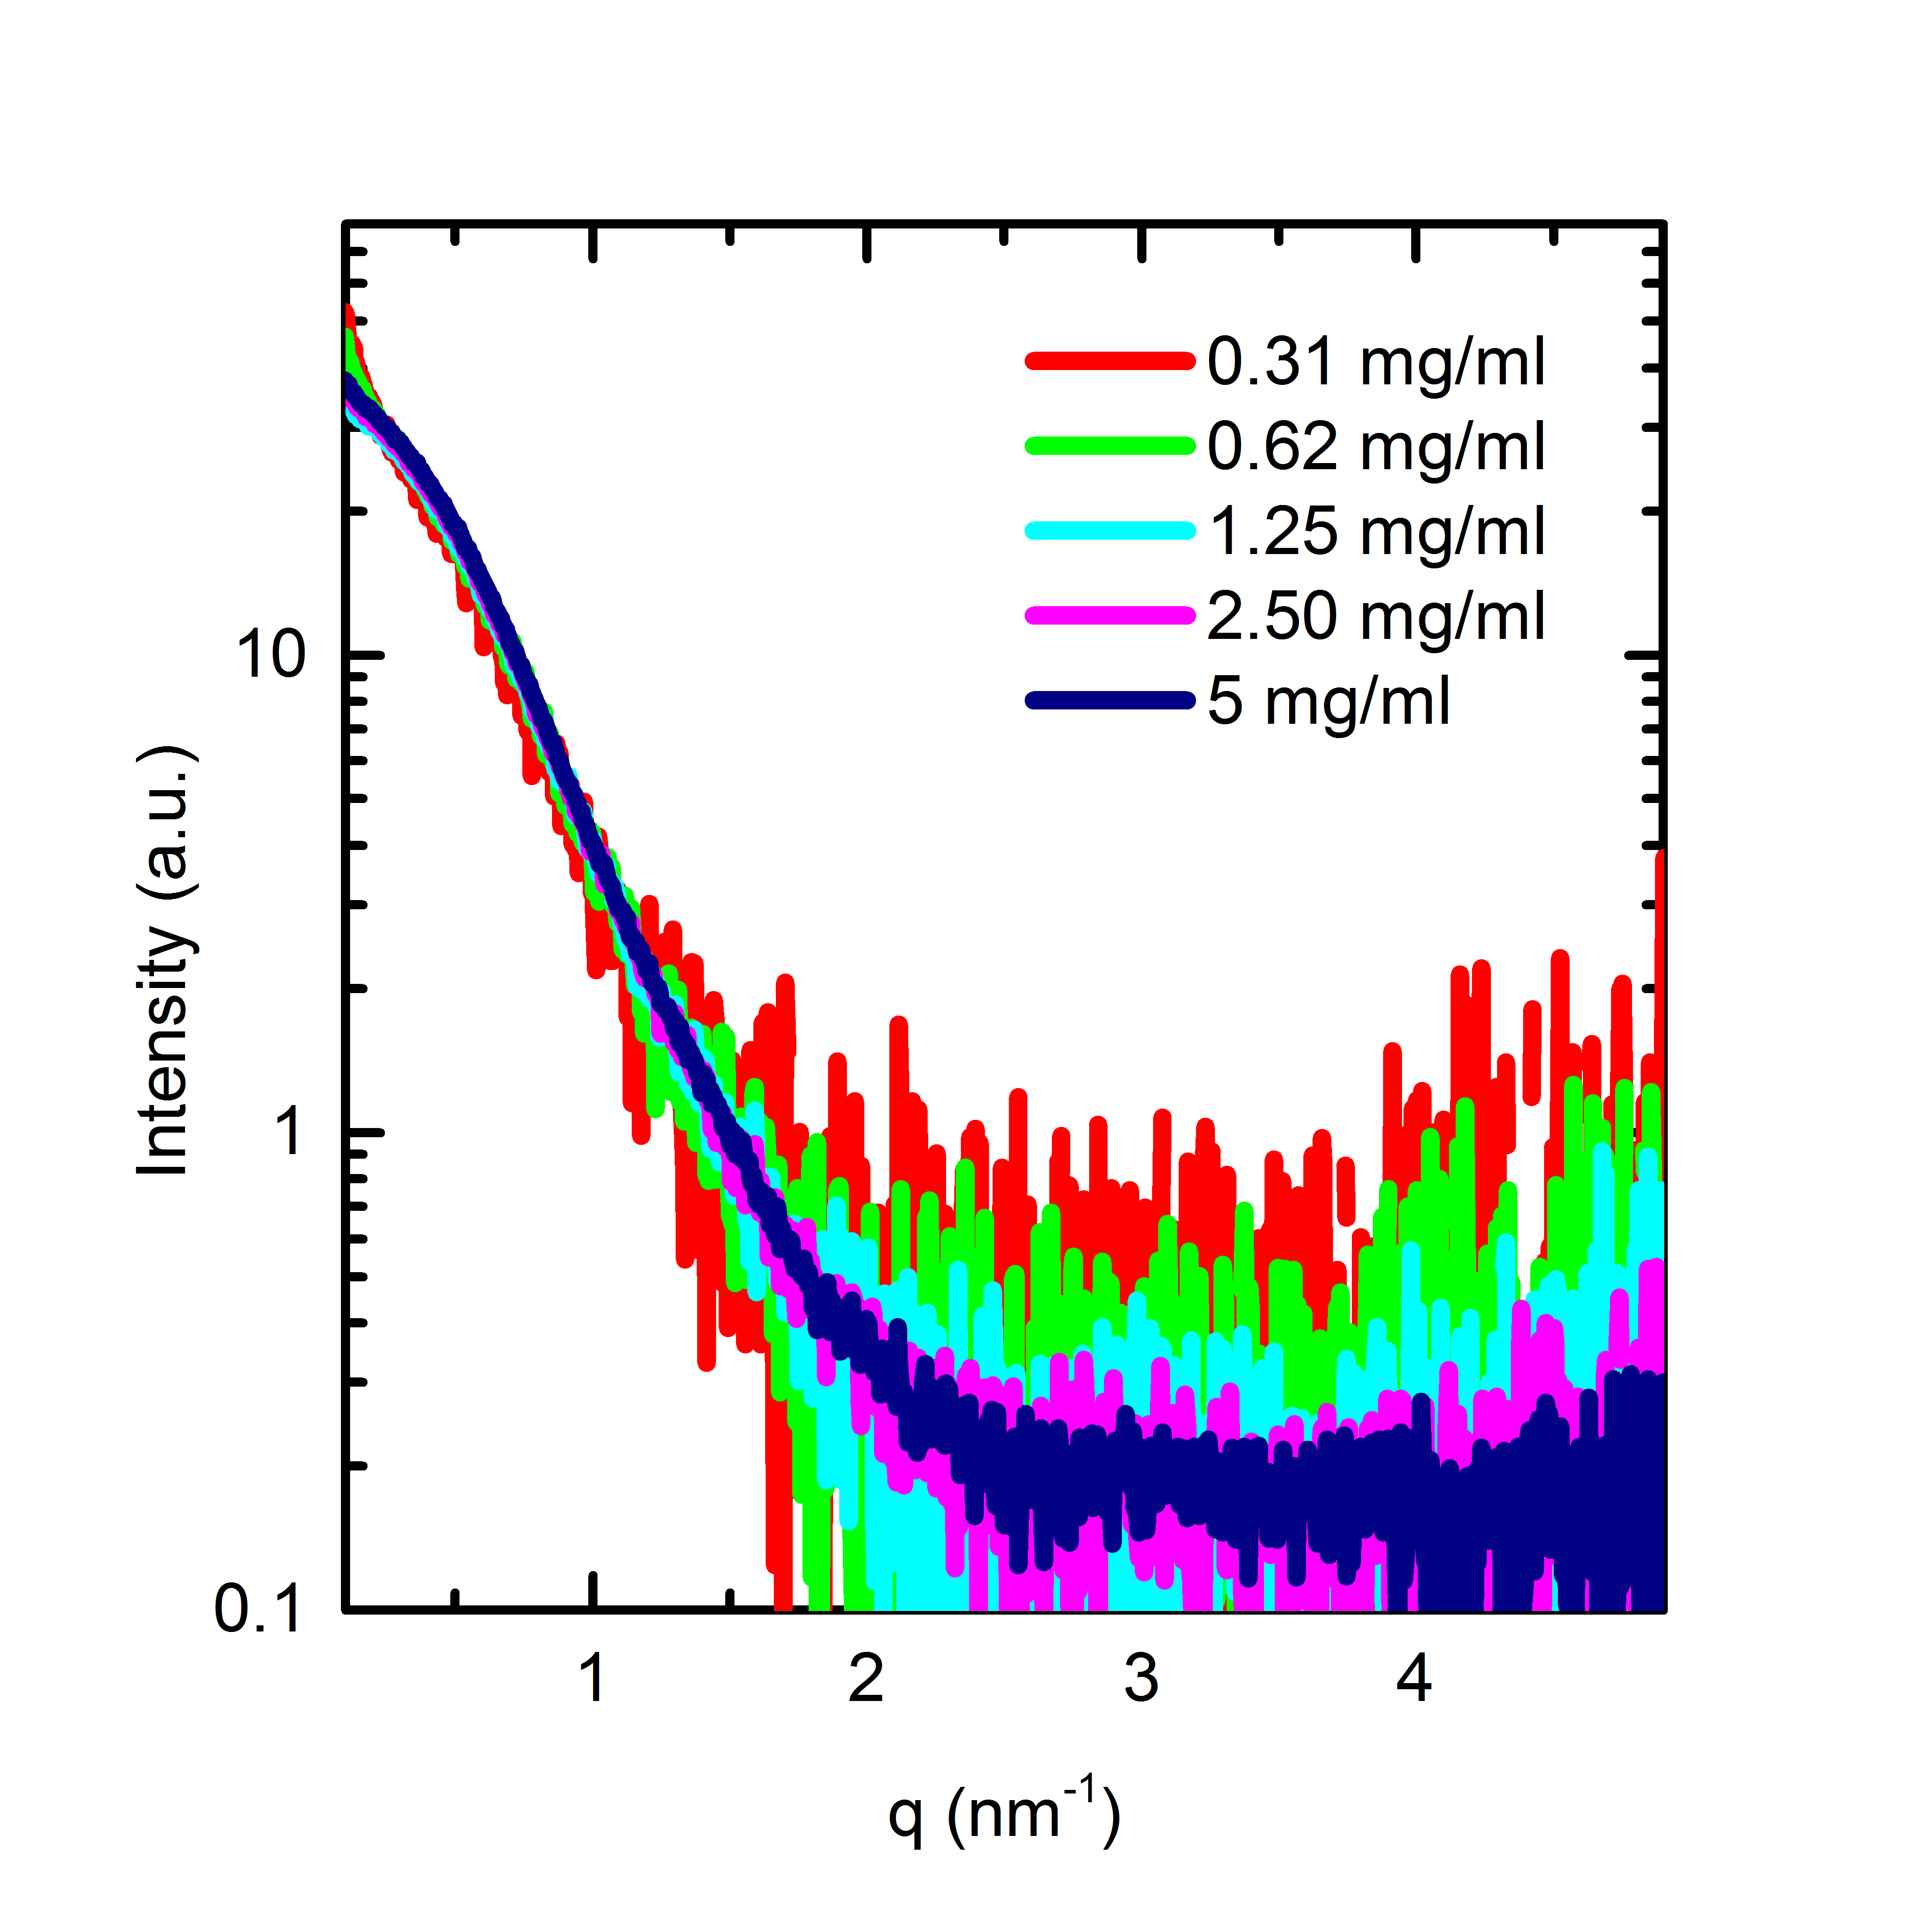
\includegraphics[width=8cm]{SCcurves.png}
\caption{Comparison of auto-subtracted SAXS patterns, of the deletion
construct of protein D5 from vaccinia virus, at different concentrations
(collected in SC mode).}
\label{fgr:SCcurves}
\end{figure}

\begin{figure}
\centering
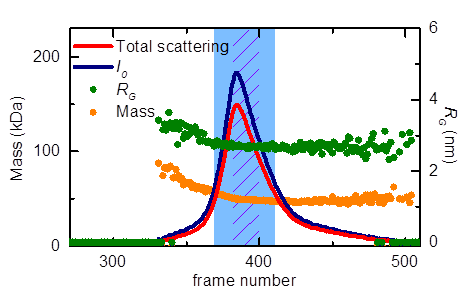
\includegraphics[width=8cm]{sec.png}
\caption{Chromatogram of a SEC-SAXS experiment on the deletion construct of
protein D5.
The plot shows total scattering intensity ($\Sigma I$), forward scattering
($I_0$), radius of gyration ($R_G$) and estimated mass from the
auto-processing as function of the frame number (take at 1 fps).
The region highlighted in blue was automatically selected for the merging of
frames, the hashed region was chosen for the manual merging.}
\label{fgr:SEC}
\end{figure}

\begin{figure}
\centering
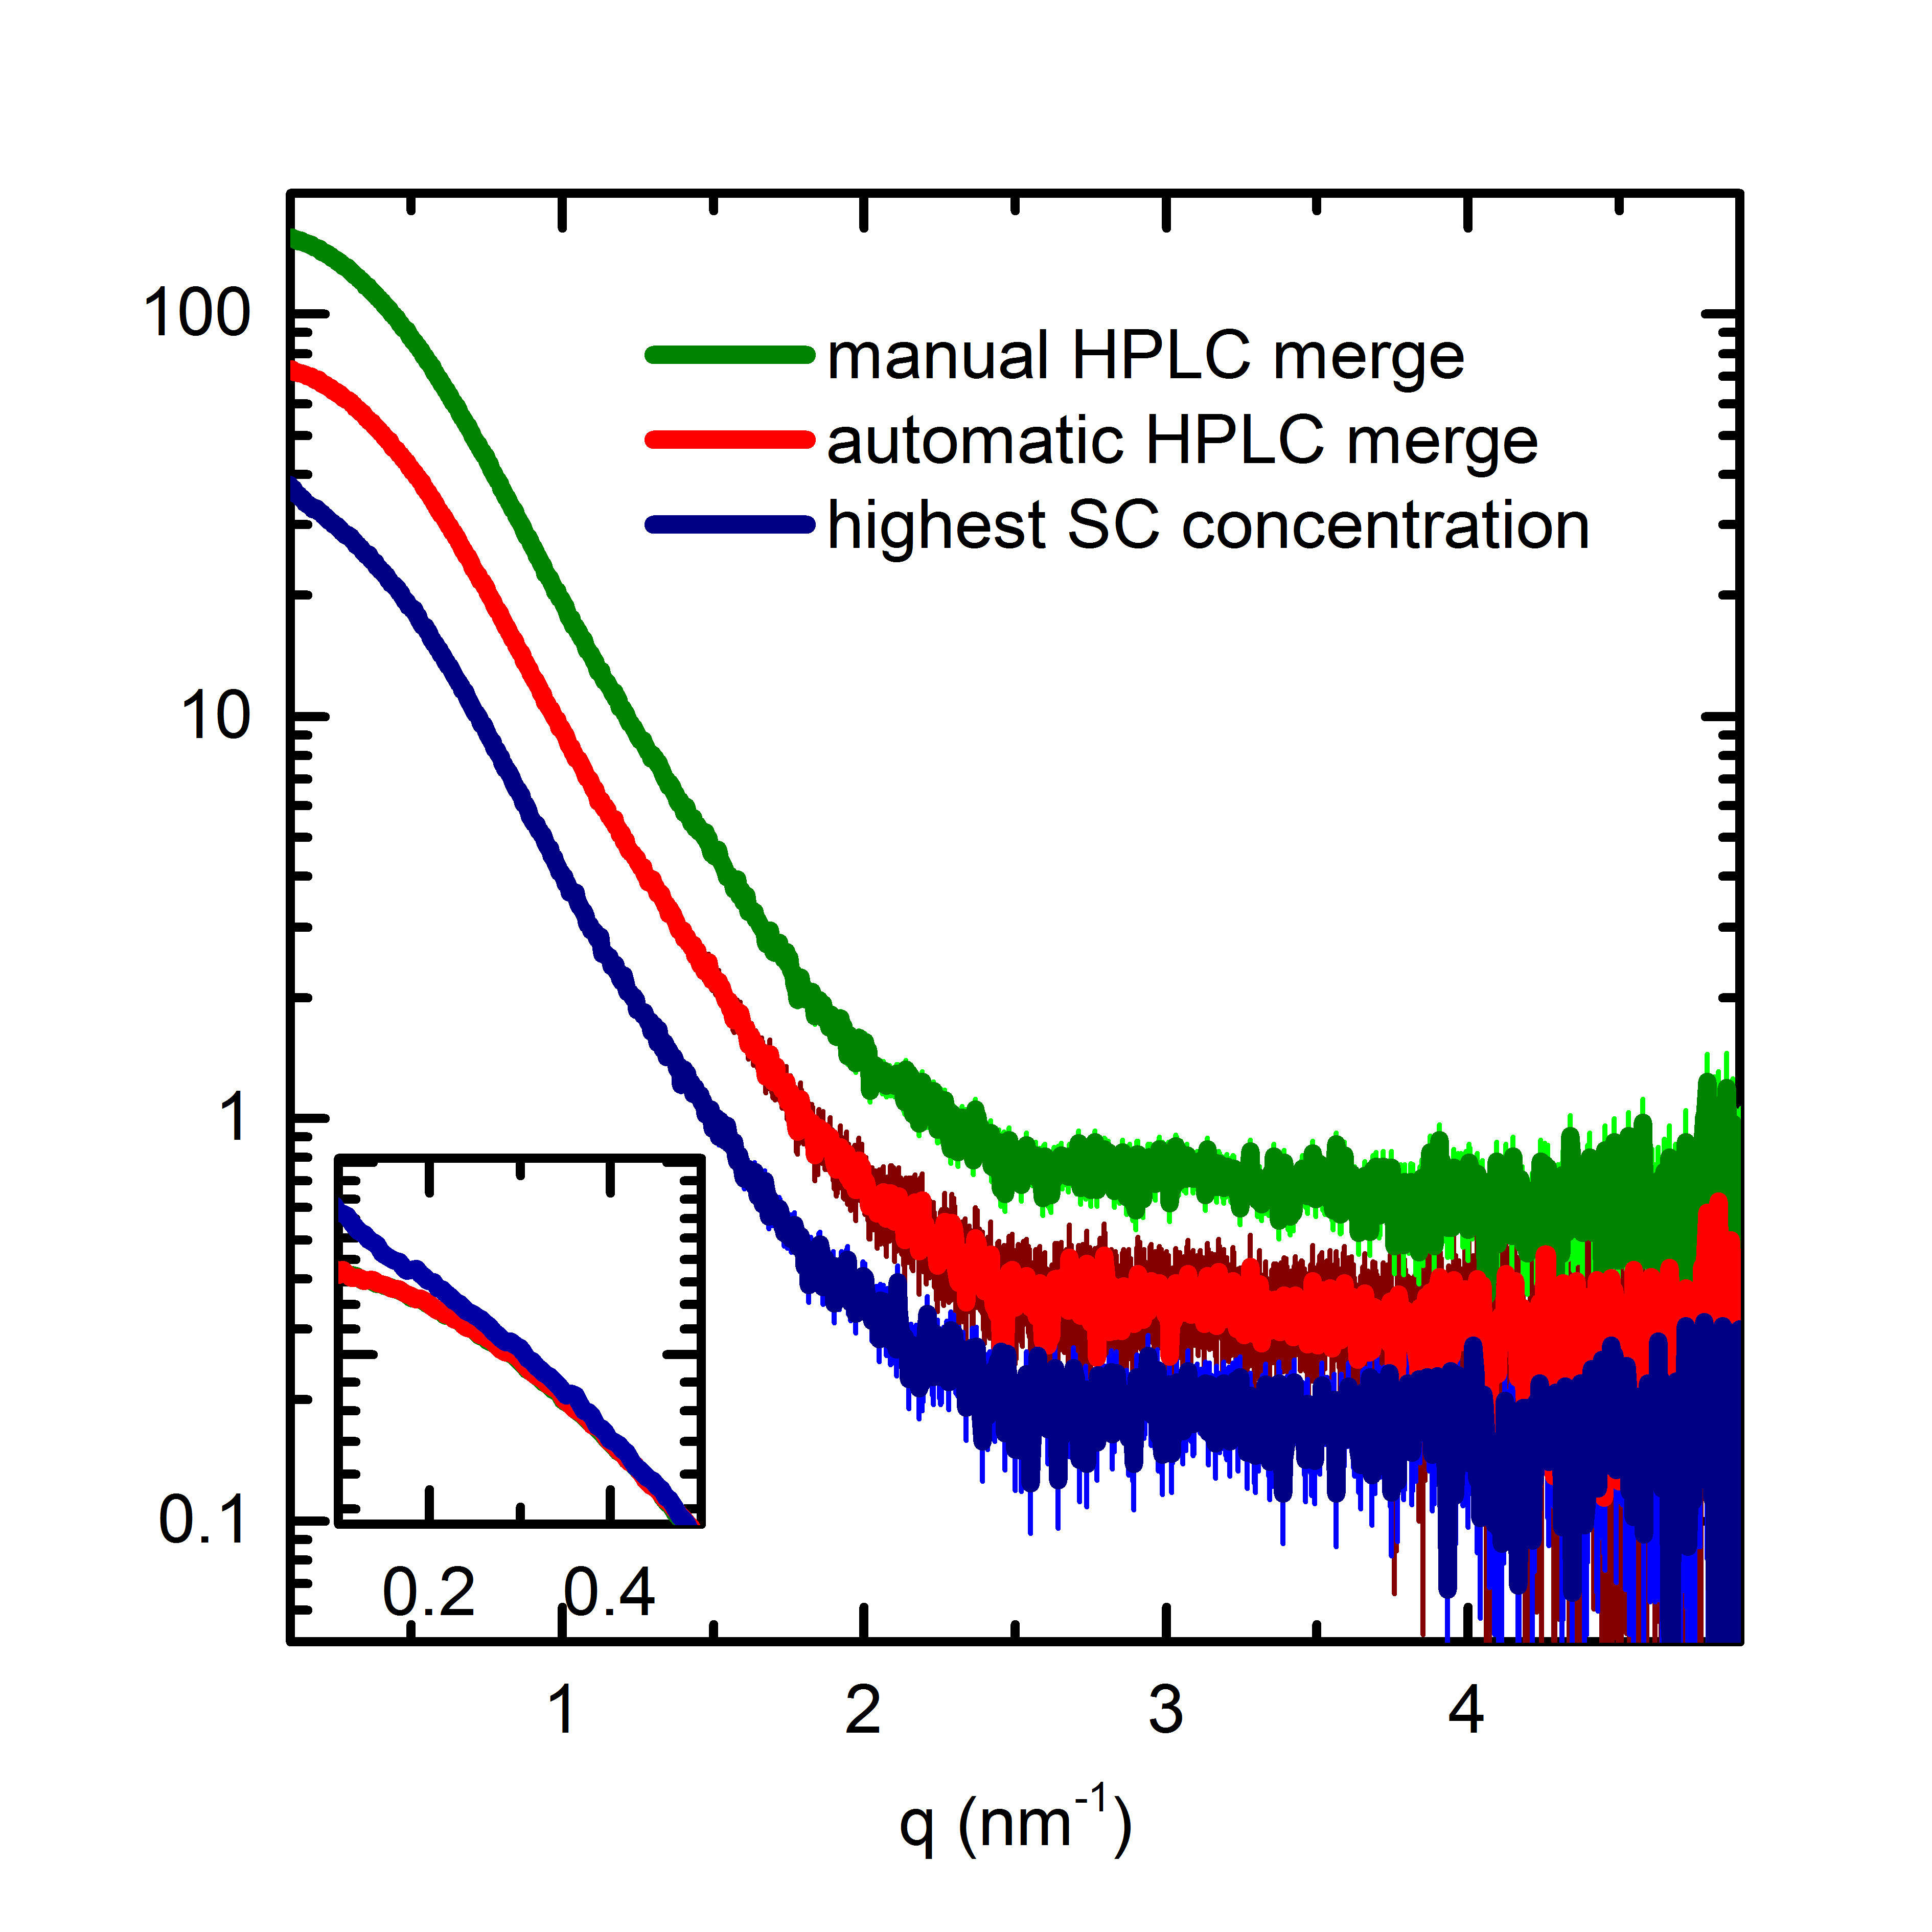
\includegraphics[width=8cm]{curves.png}
\caption{Comparison of background subtracted curves: highest concentration
collected in SC mode (blue), automatic merge (red) and manual
merge (green) of data in HPLC mode. 
The inlay shows the differences between the SC mode and HPLC mode in the
low-$q$ regime. }
\label{fgr:curves}
\end{figure}

\begin{table}
\begin{tabular}{ l c | c c c c c c }
   & $c$  & $I_{0}$  & $R_{G}$ & $D_{max}$ & $V_{P}$ & $V_{c}$ & Mass from $V_{c}$\\
	 &  (mg/ml) & (kDa) & (nm)&  (nm)&  (nm$^{3}$) & (nm$^{2}$) & (kDa)\\
\hline
Sample changer & 5.00  & 35.06 & 2.80 & 9.37  & 72.00 n& 4.18 & 50.85 \\
Sample changer & 2.50  & 34.28 & 2.83  & 9.91  & 72.08 & 4.20 & 50.15 \\
Sample changer & 1.25 & 33.58& 2.86  & 8.74  & 69.82 & 4.20 & 50.02 \\
Sample changer & 0.62  & 35.1& 2.99  & 10.48 & 73.89 & 4.40 & 52.73 \\
Sample changer & 0.31 & 35.83  & 3.26  & 8.72  & 74.42& 4.67 & 54.34 \\
HPLC, top of peak & - & 183.16 & 2.72  & -  & - & 4.08 & 49.70 \\
HPLC, merge & - & 123.89 & 2.70  & 9.46 & 69.97 & &  \\
Manual merge & - &  149.90 & 2.69 & 8.25 & & &  \\
\end{tabular}
\caption{Overview on the automatic processing results for the deletion construct of protein D5 from vaccinia virus. 
The expected mass of the protein is 45.5 kDa}
\label{tbl:results}
\end{table}


\end{document}

